\documentclass[10pt,twocolumn,letterpaper]{article}

\usepackage{textcomp}
\usepackage{listings}
\lstset{frame=lines,captionpos=b,numberbychapter=false,escapechar=§,basicstyle=\ttfamily,upquote=true}

\usepackage{iccv}
\usepackage{times}
\usepackage{epsfig}
\usepackage{graphicx}
\usepackage{amsmath}
\usepackage{amssymb}

% Thanks, http://lenaherrmann.net/2010/05/20/javascript-syntax-highlighting-in-the-latex-listings-package
\usepackage{color}
\definecolor{lightgray}{rgb}{.9,.9,.9}
\definecolor{darkgray}{rgb}{.4,.4,.4}
\definecolor{purple}{rgb}{0.65, 0.12, 0.82}

\lstdefinelanguage{JavaScript}{
  keywords={push, typeof, new, true, false, catch, function, return, null, catch, switch, var, if, in, while, do, else, case, break},
  keywordstyle=\color{blue}\bfseries,
  ndkeywords={class, export, boolean, throw, implements, import, this},
  ndkeywordstyle=\color{darkgray}\bfseries,
  identifierstyle=\color{black},
  sensitive=false,
  comment=[l]{//},
  morecomment=[s]{/*}{*/},
  commentstyle=\color{green}\ttfamily,
  stringstyle=\color{red}\ttfamily,
  morestring=[b]',
  morestring=[b]"
}

% Include other packages here, before hyperref.

% If you comment hyperref and then uncomment it, you should delete
% egpaper.aux before re-running latex.  (Or just hit 'q' on the first latex
% run, let it finish, and you should be clear).
\usepackage[pagebackref=true,breaklinks=true,letterpaper=true,colorlinks,bookmarks=false]{hyperref}
\def\sectionautorefname{Section}

% \iccvfinalcopy % *** Uncomment this line for the final submission

\def\iccvPaperID{****} % *** Enter the ICCV Paper ID here
\def\httilde{\mbox{\tt\raisebox{-.5ex}{\symbol{126}}}}

% Pages are numbered in submission mode, and unnumbered in camera-ready
\ificcvfinal\pagestyle{empty}\fi
\begin{document}

%%%%%%%%% TITLE
\title{Enabling On-the-Fly Video Scene Detection on YouTube\\ and Crowdsourcing In-Video Hot Spot Identification}

\author{Thomas Steiner, Arnaud Brousseau\\
Google Germany GmbH\\
ABC Str. 19\\
{\tt\small \{tomac, arnaudbrousseau\}@google.com}
% For a paper whose authors are all at the same institution,
% omit the following lines up until the closing ``}''.
% Additional authors and addresses can be added with ``\and'',
% just like the second author.
% To save space, use either the email address or home page, not both
\and
Ruben Verborgh, Rik Van de Walle \\
Ghent University -- IBBT, ELIS -- Multimedia Lab\\
Gaston Crommenlaan 8 bus 201, B-9050 Ledeberg-Ghent, Belgium\\
{\tt\small \{ruben.verborgh, rik.vandewalle\}@ugent.be}
}

\maketitle
% \thispagestyle{empty}

%%%%%%%%% ABSTRACT
\begin{abstract}
Video scene detection is the processor-intensive task of splitting a video into continuous scenes, with hard or soft cuts as the boundaries. In this paper, we present a client-side on-the-fly approach to this challenge based on modern HTML5-enabled Web APIs. We show how using browser extensions video scene detection can be seamlessly embedded into video platforms like YouTube.
We then explain how the generated scene set of a video drives crowdsourced identification of ``hot spots'', interesting scenes watched by many viewers. We evaluate our approach based on a set of videos that were manually split into scenes and annotated with hot~spots, indicating the potential of this technique.
\end{abstract}

%%%%%%%%% BODY TEXT
\section{Introduction}
Official statistics~\cite{youtube:stats} from YouTube~\cite{youtube}, one of the biggest online video platforms owned by Google, state that more than 13 million hours of video were uploaded during 2010, and that 35 hours of video are uploaded every single minute. Given this huge amount of video content, it becomes evident that advanced search techniques are necessary in order to retrieve the few needles from the giant haystack. Closed captions allow for keyword-based in-video search, a feature announced in 2008~\cite{googlevideo}. Searching for a phrase like ``that's a tremendous gift", a caption from Randy Pausch's famous last lecture titled \emph{Achieving Your Childhood Dreams}~\cite{pausch}, indeed reveals a link to that lecture on YouTube. If no closed captions are available, nor can be automatically generated~\cite{youtubecaptions}, keyword-based search is still available over tags, video descriptions, and titles. Presented with a potentially long list of results, preview thumbnails based on video still frames help users decide on the most promising result. YouTube lets video owners choose one out of three automatically suggested thumbnails. Until December 2008, the mechanism for the generation of such thumbnails has been simply the so-called 25/50/75 rule~\cite{youtuberule}, referring to points in the video index. This led to creative abuse of the feature to artificially increase a video's click-through rate. Currently, YouTube uses an unpublished computer vision-based algorithm for the generation of smart thumbnails on YouTube~\cite{googleresearch}.

In this paper, we introduce on-the-fly scene detection for YouTube videos as a third means besides keyword-based search and thumbnail preview for deciding on a video from the haystack. As a user starts watching a video, we detect scenes in the video by visually analyzing its content. We do this with the help of a browser extension, i.e., the whole process runs dynamically on the client-side, using the modern HTML5~\cite{w3c_html5} JavaScript APIs of the \texttt{<video>} and \texttt{<canvas>} elements. As soon as the scenes have been detected, we offer the user the choice to quickly jump into a~specific scene by clicking on a~representative still frame. \autoref{fig:screenshot} shows the seamless integration of the detected scenes into the YouTube website. We refer to such scenes of interest as \emph{hot spots}. Clicks on hot spots are tracked using a standard Web analytics service. This allows us to crowdsource hot-spot identification and suggest more accurate entry points, especially for long videos. The main contributions of this paper are the browser extension itself, the hot~spot-enabled possibility for more accurate video thumbnail selection, improved video navigability by scene access, and the potential combination with text-based semantic enrichment of metadata.

The remainder of this paper is structured as follows: \autoref{sec:related-work} presents related work in the fields of shot boundary detection and semantic enrichment of user-generated metadata on YouTube, \autoref{sec:details-of-algo} explains our scene detection algorithm in detail, \autoref{sec:implementation} outlines the implementation details of our browser extension, \autoref{sec:evaluation} shows an evaluation of first preliminary results. Finally, \autoref{sec:future-work-conclusion} gives an outlook on future work and ends the paper with a~\mbox{conclusion}.

\begin{figure*}
\begin{center}
   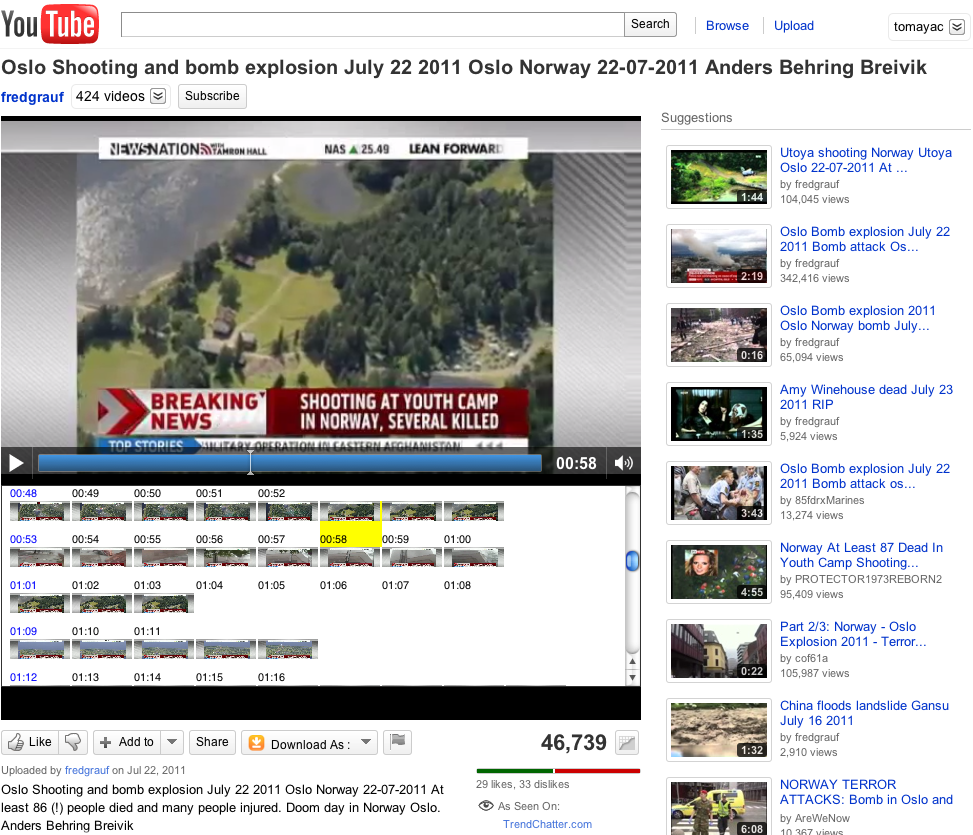
\includegraphics[width=0.8\linewidth]{./resources/screenshot.png}
\end{center}
   \caption{Screenshot of the YouTube browser extension, showing the different detected scenes.}
\label{fig:screenshot}
\end{figure*}

\section{Related Work} \label{sec:related-work}
We consider related work in the strictly related field of shot boundary detection and in the loosely related field of semantic enrichment of user-generated metadata on YouTube.

\subsection{Shot Boundary Detection}
Video fragments consist of shots, which are sequences of consecutive frames from a single viewpoint, representing a continuous action in time and space. The topic of shot boundary detection has already been described extensively in literature. While some specific issues still remain (notably gradual transitions and false positives due to large movement or illumination changes), the problem is considered resolved for many cases~\cite{Hanjalic2002, Yuan2007}. Below, we present an overview of several well-known categories of techniques.

Pixel comparison methods~\cite{Hampapur1994, Zhang1993} construct a discontinuity metric based on differences in color or intensity values of corresponding pixels in successive frames. This dependency on spatial location makes this technique very sensitive to (even global) motion. Various improvements have been suggested, such as prefiltering frames~\cite{Zhang1995}, but pixel-by-pixel comparison methods proved inferior in the end and have steered research towards other directions.

A related method is histogram analysis~\cite{Smeaton1999}, where changes in frame histograms are used to justify the boundaries of shots. Their insensitivity to spatial information within a frame makes histograms less prone to partial and global movements in a scene. We can argue as a drawback that even visually very dissimilar frames can have similar overall histograms. For example, different shots in the same scene can be difficult to distinguish because of similar color information.

As a compromise, a third group of methods consists of a trade-off between the above two techniques~\cite{Ahmed1999}. Different histograms of several, non-overlapping blocks are calculated for each frame, thereby categorizing different regions of the image with their own color-based, space-invariant fingerprint. The results are promising, while computational complexity is kept to a minimum, which is why we have chosen a variation on this approach in this paper.

Other approaches to shot boundary detection include the comparison of mean and standard deviations of frame intensities~\cite{Lienhart1999}. Detection using other features such as edges~\cite{Zabih1995} and motion~\cite{Bouthemy1997} have also been proposed. However, Gargi \emph{et~al.}\ have shown that these more complex methods do not necessarily outperform histogram-based approaches~\cite{Gargi2000}. A detailed overview and comparison can be found in Yuan~\emph{et~al.}~\cite{Yuan2007}. 

Another interesting track is shot boundary detection in the compressed domain~\cite{Yeo1995}, which is especially relevant for online video, as compression plays a major part herein. Unfortunately, even though this article focuses on online video, client-side manipulation of the raw, compressed stream would introduce a lot of computational overhead and make our implementation codec-dependent.

\subsection{Semantic Enrichment of User-Generated Metadata on YouTube}
Choudhury \emph{et~al.}~\cite{Choudhury:YouTube} describe a framework for the semantic enrichment, ranking, and integration of Web video tags using Semantic Web technologies. In order to enrich the oftentimes sparse user-generated tag space, they use metadata like the recording time and location, or the video title and description, but also social features such as related videos and playlists a video appears in. Next, they rank the tags by their co-occurrence and, as a final step, interlink with DBpedia~\cite{Bizer:DBpedia}. While the semantic enrichment of YouTube metadata is of little help for the actual detection of scenes in a video, it still can help to visually ``iconify" them. For example, if it is known that a certain scene is about the DBpedia concept of the company Apple, Inc., this scene can then be visually represented by an icon in form of the Apple logo, in addition to the scene still frames.

Steiner and Hausenblas~\cite{semwebvid} describe a Web application that allows for the automatic generation of Resource Description Framework (RDF) video descriptions based on user-generated metadata such as title, description, tags, and closed captions. They enrich this textual information via multiple Natural Language Processing Web services in parallel in order to extract named entities. The detected named entities are interlinked with DBpedia concepts. While their detected named entities are explicitly anchored to a point in the video thanks to the closed captions, our scene detection framework can instead anchor named entities to scenes, which is context-wise oftentimes the better option.

Finally, Gao \emph{et~al.}~\cite{Gao:2009} propose a theme-based thumbnail selection algorithm that explicitly models the visual characteristics of the underlying semantic video theme. This semantic model is constructed by finding the common features of relevant visual samples, which are obtained by querying a visual database with keywords associated with the video. Synergies between the approaches~\cite{Choudhury:YouTube,Gao:2009,semwebvid} and our current approach of scene detection with crowdsourced hot spot identification are possible.

\section{Scene Detection Algorithm} \label{sec:details-of-algo}
In this Section, we discuss our scene detection algorithm, which falls in the category of histogram-based algorithms.  Since visually dissimilar video frames can have similar overall histograms, we also take into account local histograms. 
We therefore split our video frames in freely configurable rows and columns, hence, lay over a grid of tiles over the frames. The user interface currently allows for anything from $1 \times 1$ to $20 \times 20$ layouts. For each step we examine a frame $n$ and its direct predecessor frame $n - 1$.

Apart from the obvious per-tile histogram average distance, our frame distance function further considers a freely configurable number of to-be-examined most different or similar tiles. This is driven by the observation that different parts of the video have different intensities of color changes, dependent on the movements from frame to frame. The idea is thus to increase the influence of movements in the frame distance function, and to decrease the influence of static parts. This can be best illustrated with the example given in \autoref{fig:algorithm}. The anchorman is framed by two news tickers, one above, and one below his head. The many red boxes indicate movements on the tiles with the news tickers.
In contrast, the top-upper gray background of the studio wall is entirely static, having many green boxes in consequence. Besides the anchorman's movements, resulting in red boxes around his face, there are many screens with live video behind him, explaining the remaining red boxes. For this example, we used a grid layout of $20 \times 20$ (which implies $\mathit{numTiles} = \mathit{rows} \times \mathit{columns} = 400$), and a number $\mathit{nDiffSim}$ of most different or similar tiles of~$133$ (which corresponds to $\mathit{rows} \times {columns}\,/\,3$). In our frame distance function, we apply boosting and limiting factors to the most different and most similar tiles respectively. In our example we worked with a $\mathit{boostingFactor}$ of~$2$, which doubles the impact of the most different tiles, and a $\mathit{limitingFactor}$ of~$0.5$, which of course halves the impact of the most similar tiles. The complete algorithm can be seen in \autoref{code:algorithm}.

\begin{figure}
\begin{center}
   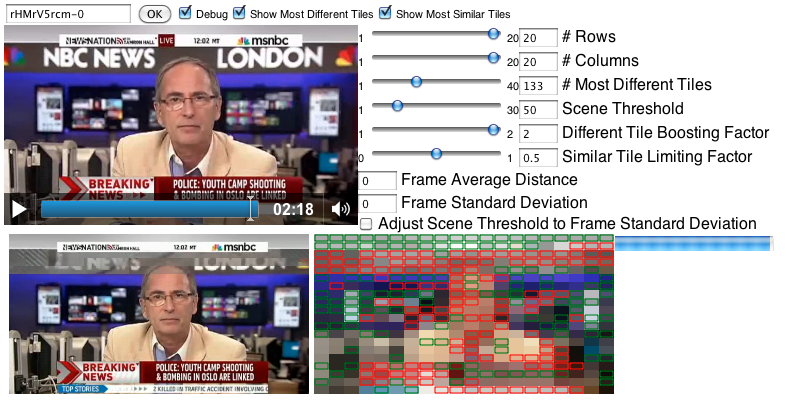
\includegraphics[width=1.0\linewidth]{./resources/algorithm.png}
\end{center}
   \caption{Debug view of the scene detection process. Red boxes highlight tiles with the most differences to the previous frame, green boxes those with most similarities.}
\label{fig:algorithm}
\end{figure}

\begin{lstlisting}[caption=Pseudocode for our scene detection algorithm., label=code:algorithm, float]
dist = []
for frame in frames
  i = frame.index
  avgHisto[i] = getAvgHisto(frame)
  dist[i] = histoDist(frame, frame[i-1])

  mostDiffTiles =
    getMostDiffTiles(dist[i], nDiffSim)
  mostSimTiles =
    getMostSimTiles(dist[i], nDiffSim)

  for tile in tiles
    factor = 1
    if tile in mostDiffTiles
      factor = boostingFactor
    if tile in mostSimTiles
      factor = limitingFactor
    avgHisto[i][tile] =
      avgHisto[i][tile] §$\times$§ factor
avgDist = avg(dist)
\end{lstlisting}

We have made some basic statistic examinations of the frame distance data and experimentally found out that, while the average frame distance $$\mathit{avgDist} = \frac{1}{\mathit{numTiles}}\sum_{n=1}^{\mathit{numTiles}}\mathit{avgHisto}_{n}$$ is very intuitive to human beings, far more value lies in the standard deviation, based on the definition of the average distance. $$\sqrt{\frac{1}{\mathit{numTiles}}\sum_{n=1}^{\mathit{numTiles}}(\mathit{avgHisto}_{n} - \mathit{avgDist})^{2}}$$ We can actually directly use the value of the standard deviation as a scene splitting threshold value to come to very accurate scene splitting results. We found the boosting and limiting factors to have overall a positive scene splitting quality impact on more lively videos, and a negative quality impact on more monotone videos. The results are optimal if, after changing either the boosting or the limiting factor, the scene splitting threshold is adapted to the new standard deviation.

\section{Implementation Details} \label{sec:implementation}
We begin this Section with an overview of the technologies used, namely we introduce Google Chrome extensions for the Google Chrome browser, and give a brief summary of the Web analysis solution Google Analytics.

\subsection{Google Chrome Extensions}
Google Chrome extensions~\cite{chromeextensions} are small software programs that users can install to enrich the browsing experience with the Google Chrome~\cite{chrome} browser. They are written using a combination of standard Web technologies, such as HTML, JavaScript, and CSS. Chrome extensions get usually (but not necessarily) distributed through the Chrome Web Store~\cite{chromewebstore}. There are several types of extensions, for this paper we focus on extensions based on so-called content scripts. Content scripts are JavaScript programs that run in the context of Web pages via dynamic code injection. By using the standard Document Object Model (DOM), they can read or modify details of the Web pages a user visits.

\subsection{Google Analytics}
Google Analytics~\cite{googleanalytics} is Google's Web analysis solution allowing for detailed statistics about the visitors of a website. The software is implemented by adding an invisible snippet of JavaScript code on the to-be-tracked pages of a website. This code collects visitor data through a request for a specific $1x1$ pixel image, during which the page and user data is reported back in the query part of the image's URL. In addition to that, the snippet sets a first party cookie on visitors' computers in order to store anonymous information such as the timestamp of the current visit, whether the visitor is a new or returning visitor, and the referrer of the website that the visitor came from.

\subsection{Video Analysis Process}
As outlined before, the complete video analysis process happens fully on the client side. We use modern HTML5~\cite{w3c_html5} JavaScript APIs of the HTML \texttt{<video>} and \texttt{<canvas>} elements. Our extension gets activated as soon as the user enters a page that matches the URL pattern \url{http://www.youtube.com/watch*}, i.e., YouTube video watch pages. By default, YouTube uses Flash-encoded~\cite{flash} videos that are not programmatically accessible, however, via an API used by the YouTube \texttt{<iframe>} embed code~\cite{youtubeiframe}, we can retrieve the HTML5 versions of a video that are encoded in any of the HTML5-supported video codecs~\cite{html5video}. In order to obtain a video still frame from the \texttt{<video>} element at the current video position, we use the \texttt{drawImage()} function of the 2D context of the \texttt{<canvas>} element, which as its first parameter accepts a \texttt{<video>} element. We then analyze the video frame's pixels tile-wise and calculate the histograms. The pitfall with this approach is that in order to retrieve the tile-wise pixel data from the 2D context of the \texttt{<canvas>}, we need the \texttt{getImageData()} function to which the so-called Same Origin Policy~\cite{sameoriginpolicy} applies. This means that the \texttt{<canvas>} cannot use the video data directly  from YouTube, but has to use a proxied version on the same domain, which effectively means that we have to temporarily store the video on a proxy server. For processing speed reasons, we currently limit our approach to a resolution of one second, i.e., for each analysis step seek the video in second-steps. We then calculate the frame distances as outlined in Section~\ref{sec:details-of-algo}. For each frame, we generate an \texttt{<img>} element with a base64-encoded data URI~\cite{datauri} representation of the video frame's data that later gets injected into the YouTube watch page's DOM tree, as can be seen in \autoref{fig:screenshot}. Each of the \texttt{<img>} elements has a registered JavaScript event handler that upon click triggers two actions: first, the video seeks to the corresponding time, and second, the frame gets tracked as a hot spot in the video, i.e., as a scene of interest. We therefore use Google Analytics event tracking~\cite{analyticsevent}, a sample hot spot tracking event code snippet is shown in Listing~\ref{code:event}.

\begin{lstlisting}[caption=JavaScript hot spot event tracking code snippet. The \texttt{\_gaq} object refers to the Google Analytics event tracking queue., label=code:event, float=t, frame=single, language=JavaScript]
_gaq.push(['filmstrip._trackEvent', 
    'seek', // event type (string)
    'Bo2p82aTQzo', // video ID (string)
     '64' // time cue (string)
]);
\end{lstlisting} 

\section{Evaluation} \label{sec:evaluation}
Detecting scenes on-the-fly of streaming video comes with its very own challenges. First, and most obviously, it is a question of streaming speed. We have to stream two videos in parallel: on the one hand the video that the user sees upon navigating to a YouTube watch page, and on the other hand the video that is being used in the background for the analysis process. Note that due to the Same Origin Policy~\cite{sameoriginpolicy} we are indeed forced to stream two copies of the video to two different destinations, as the analysis process necessarily has to be performed on the same domain as the scene analysis code, it cannot run on the same domain as the YouTube video. Especially with high-definition (HD) video this can be very demanding. There is some room for improvement by requesting a low-density (LD) version of the video for the analysis in the background, however, with the current implementation constraints it will always be two streams. Second, and somehow related, rendering the two streams is a very processor-intensive task. We do not attach the background \texttt{video} element to the DOM tree to safe some CPU cycles, however, the video still needs to be seeked to each frame in second-steps, be processed, and be streamed. Even on a rather higher-end consumer laptop (our configuration MacBook Pro, Intel Core 2 Duo 2,66 GHz, 8 GB RAM), the process of analyzing and in parallel displaying a $1280x720$ HD video of media type video/mp4; codecs="avc1.64001F, mp4a.40.2" causes an average CPU load of about 70\%, which lets the laptop cooling fans spin up hearibly\ldots In order to keep up with the stream, i.e., \textit{``[\ldots] when the playback rate is not exactly 1.0, hardware, software, or format limitations can cause video frames to be dropped [\ldots]"}~\cite{whatwgvideo}. In practice this causes the analysis environment to be far from optimal.

\subsection{Video Scene Detection}
With this rather lengthy preamble, in Table~\ref{table:results} we present some first preliminary results. The analysis settings for the experiment were as follows: $rows = 20$, $columns = 20$, $nDiffSim = 133$, $boostingFactor = 2.0$, $limitingFactor = 0.5$, $sceneThreshold = standardDeviation$. We had two humans split 10 randomly selected videos into scenes, and afterwards compared their scene classification with the automatically generated one. We counted \emph{matches} (humans and machine agreed), \emph{misses} (the humans detected a scene change, the machine did not), and \emph{false positives} (the machine detected a scene change, the humans did not). 

\begin{table}
\begin{center}  
    \begin{tabular}{ | l | l | l | l |}
    \hline
    \textbf{Video ID} & \textbf{Matches} & \textbf{Misses} & \textbf{False Positives} \\ \hline
    nCAZIVoE\_AQ & 8 & 1 & 1 \\ \hline
    9cZk267ezLw & 8 & 1 & 0	 \\ \hline
    vqVdm6zMmRc & 4 & 12 & 2 \\ \hline
    kFAJ-XAF7oM & 5 & 3 & 1 \\ \hline
    118fTtOKoc4 & 10 & 9 & 3 \\ \hline
    xyLHGlUN9rM & 16 & 2 & 8 \\ \hline
    iqqLmdLecJw & 6 & 0 & 4 \\ \hline
    5eIqe3tPczE & 5 & 0 & 4 \\ \hline
    noeTBLB30ac & 9 & 3 & 0 \\ \hline
    \hline
    \end{tabular}
\end{center}
\caption{Manual scene detection compared to automatic scene detection.}
\label{table:results}
\end{table}

Having a closer look at the source videos and interpreting these results, we can see that most misses are due to frame drops in the background analysis video, especially with HD video material. Given the preamble, this is not surprising. In addition to that, our human scene detectors counted rapid scene changes far beyond one-second-resolution, as for example in the Harry Potter movie trailer (vqVdm6zMmRc). Already by design, our approach cannot compete with this fine level of granularity, nor does it make sense trying to get there given our objectives of allowing for video hot spot-enabled more accurate video thumbnail selection, and improved video navigability by scene access. A more critical problem was that sometimes when a video could not be seeked to the desired time, the still frame remained static, an effect that for some reason reproducibly occurred in the Sky News report video on Amy Winehouse's funeral (iqqLmdLecJw). This seems to be more a problem with the video encoding and the key frames rather than a problem of our code. 

\subsection{Hot Spot Identification}
We had two humans look at scene frames of 30 randomly selected videos and asked them to click on frames they found visually appealing. This resulted in overall just over 200 hot spots being tracked via Analytics. After analyzing the hot spots manually, we found that the humans used them in two ways: first, in a \emph{navigational way}, and second, in an \emph{interest-based way}. For the navigational way, the humans jumped either back to the beginning of the video (the trivial case), or skipped intros, which could be repeatedly observed in several videos, e.g., in the Kernkraft 400 -- Zombie Nation music video (z5LW07FTJbI) that has an annoying intro in the first 12 seconds. For the second interest-based category, the humans were attracted by promising frames, e.g., the fire-spitting dragon in the Harry Potter trailer at position 6 seconds, that both humans clicked twice, or the Fail Blog clip Responsible Sibling Fail (kFAJ-XAF7oM), where both humans repeatedly watched a poor kid get hit hard on the head by a soccer ball.

If we compared the detected hot spot video frames with the actually displayed YouTube video thumbnails, we could observe room for improvement. Based on the human testers whom we first showed the videos, and then blindly asked them to decide on the most appropriate thumbnail from a set of the actual thumbnail and video frames from video hot spots reported by different users, in close to 90\% of the cases the testers decided for a video hot spot frame, and not for the YouTube thumbnail. 

\section{Future Work and Conclusion} \label{sec:future-work-conclusion}
In this paper, we have first presented related work in the field of video shot boundary detection and the semantic enrichment of user-generated metadata on YouTube. In continuation, we have introduced our scene detection algorithm, and have outlined its implementation details regarding the two used tools Analytics and Chrome extensions, and the extension's underlying HTML5 JavaScript APIs. In a last step we have evaluated our approach in the two categories video scene detection and hot spot identification.

Future work will be in a first step to improve the analysis speed by a more dynamic selection of the to-be-analyzed background video file. Most videos are available in several resolutions, both LD and HD. We will have to check in how far analysis results differ for the various versions. In a second step, we will work on coming up with more advanced heuristics for the various user-definable options in the analysis process. The options can be seen in \autoref{fig:algorithm}. While there probably is no such thing as \emph{the} optimal configuration for whatever video, there are probably some key indicators to look out for, such as $x < averageDistance  < y$, $standardDeviation - averageDistance < x$, always in dependence on the values of the values of $boostingFactor$, $limitingFactor$, $rows$, and $columns$. For our first experimental preliminary results there is some evidence that simpler is in most cases good enough, i.e., a higher number of $rows$ and $columns$ than two does not necessarily lead to more accurate scene detection results, the same applies to the number of to-be-considered most different or similar tiles $nDiffSim$. We even had cases where not treating those tiles differently at all, i.e., setting $boostingFactor  = limitingFactor = 1$, led to better results. In a third step, we want to combine our approach with elements of the approaches of Choudhury et al., Steiner and Hausenblas, and Gao et al.~\cite{Choudhury:YouTube,Gao:2009,semwebvid}. We are convinced of the joint power of low-level visual analysis and the high-level semantic text-based analysis. In a forth step, we might consider proceeding with a server-side, rather than a client-side approach, albeit given the current YouTube upload rates~\cite{youtube:stats} crowdsourced client-side processing seems like a viable option, at least for the millions of hours of already existing video material.

Concluding, we have some first promising results, especially with regards to hot spot identification, which in the future could serve for more accurate entry point suggestions in long videos, or enable skip marks in videos with intros. Also for the suggestion of video thumbnails, a combined crowdsourced hot spot-based approach could lead to more accurate results than the current purely computer vision-based approach~\cite{googleresearch}. For scene identification, some challenges remain, especially given the streaming issues we observed. Nonetheless, the generated results albeit not perfect allowed for more focused video seeking than blindly jumping into random points in the video.

{\small
\bibliographystyle{ieee}
\bibliography{artemis2011}
}

\end{document}